% Figure s02f05_flatbands (Session 2): flat bands in the Lieb and kagome lattices.
% The image is rendered by figures/blender/s02f05_flatbands.py; the coordinates of the labels come from
% figures/blender/out/s02f05_flatbands_anchors.tex. Build with figures/blender/build_figure.sh s02f05_flatbands.
\documentclass[11pt,tikz,border=0pt]{standalone}
\usepackage[T1]{fontenc}
\usepackage{amsmath,amssymb,graphicx,bm}
\usepackage{xcolor}
\usetikzlibrary{arrows.meta,calc}
% The three label colors of the figures, with the same values as in src/figures_preamble.tex.
\definecolor{aqmaccent}{RGB}{31,78,121}
\definecolor{aqmbroken}{RGB}{168,42,34}
\definecolor{aqmmuted}{RGB}{125,125,125}

\newlength{\figw}\setlength{\figw}{15.6cm}   % the text width of the notes (A4, 2.7 cm margins)

\begin{document}
\begin{tikzpicture}[lbl/.style={font=\small, inner sep=1.5pt}, pnl/.style={font=\small\bfseries, inner sep=1.5pt}]
  \begin{scope}[shift={(0.00cm,0)}]
    \setlength{\figw}{2.9cm}
    \node[overlay, anchor=south west, inner sep=0pt] at (0,0)
      {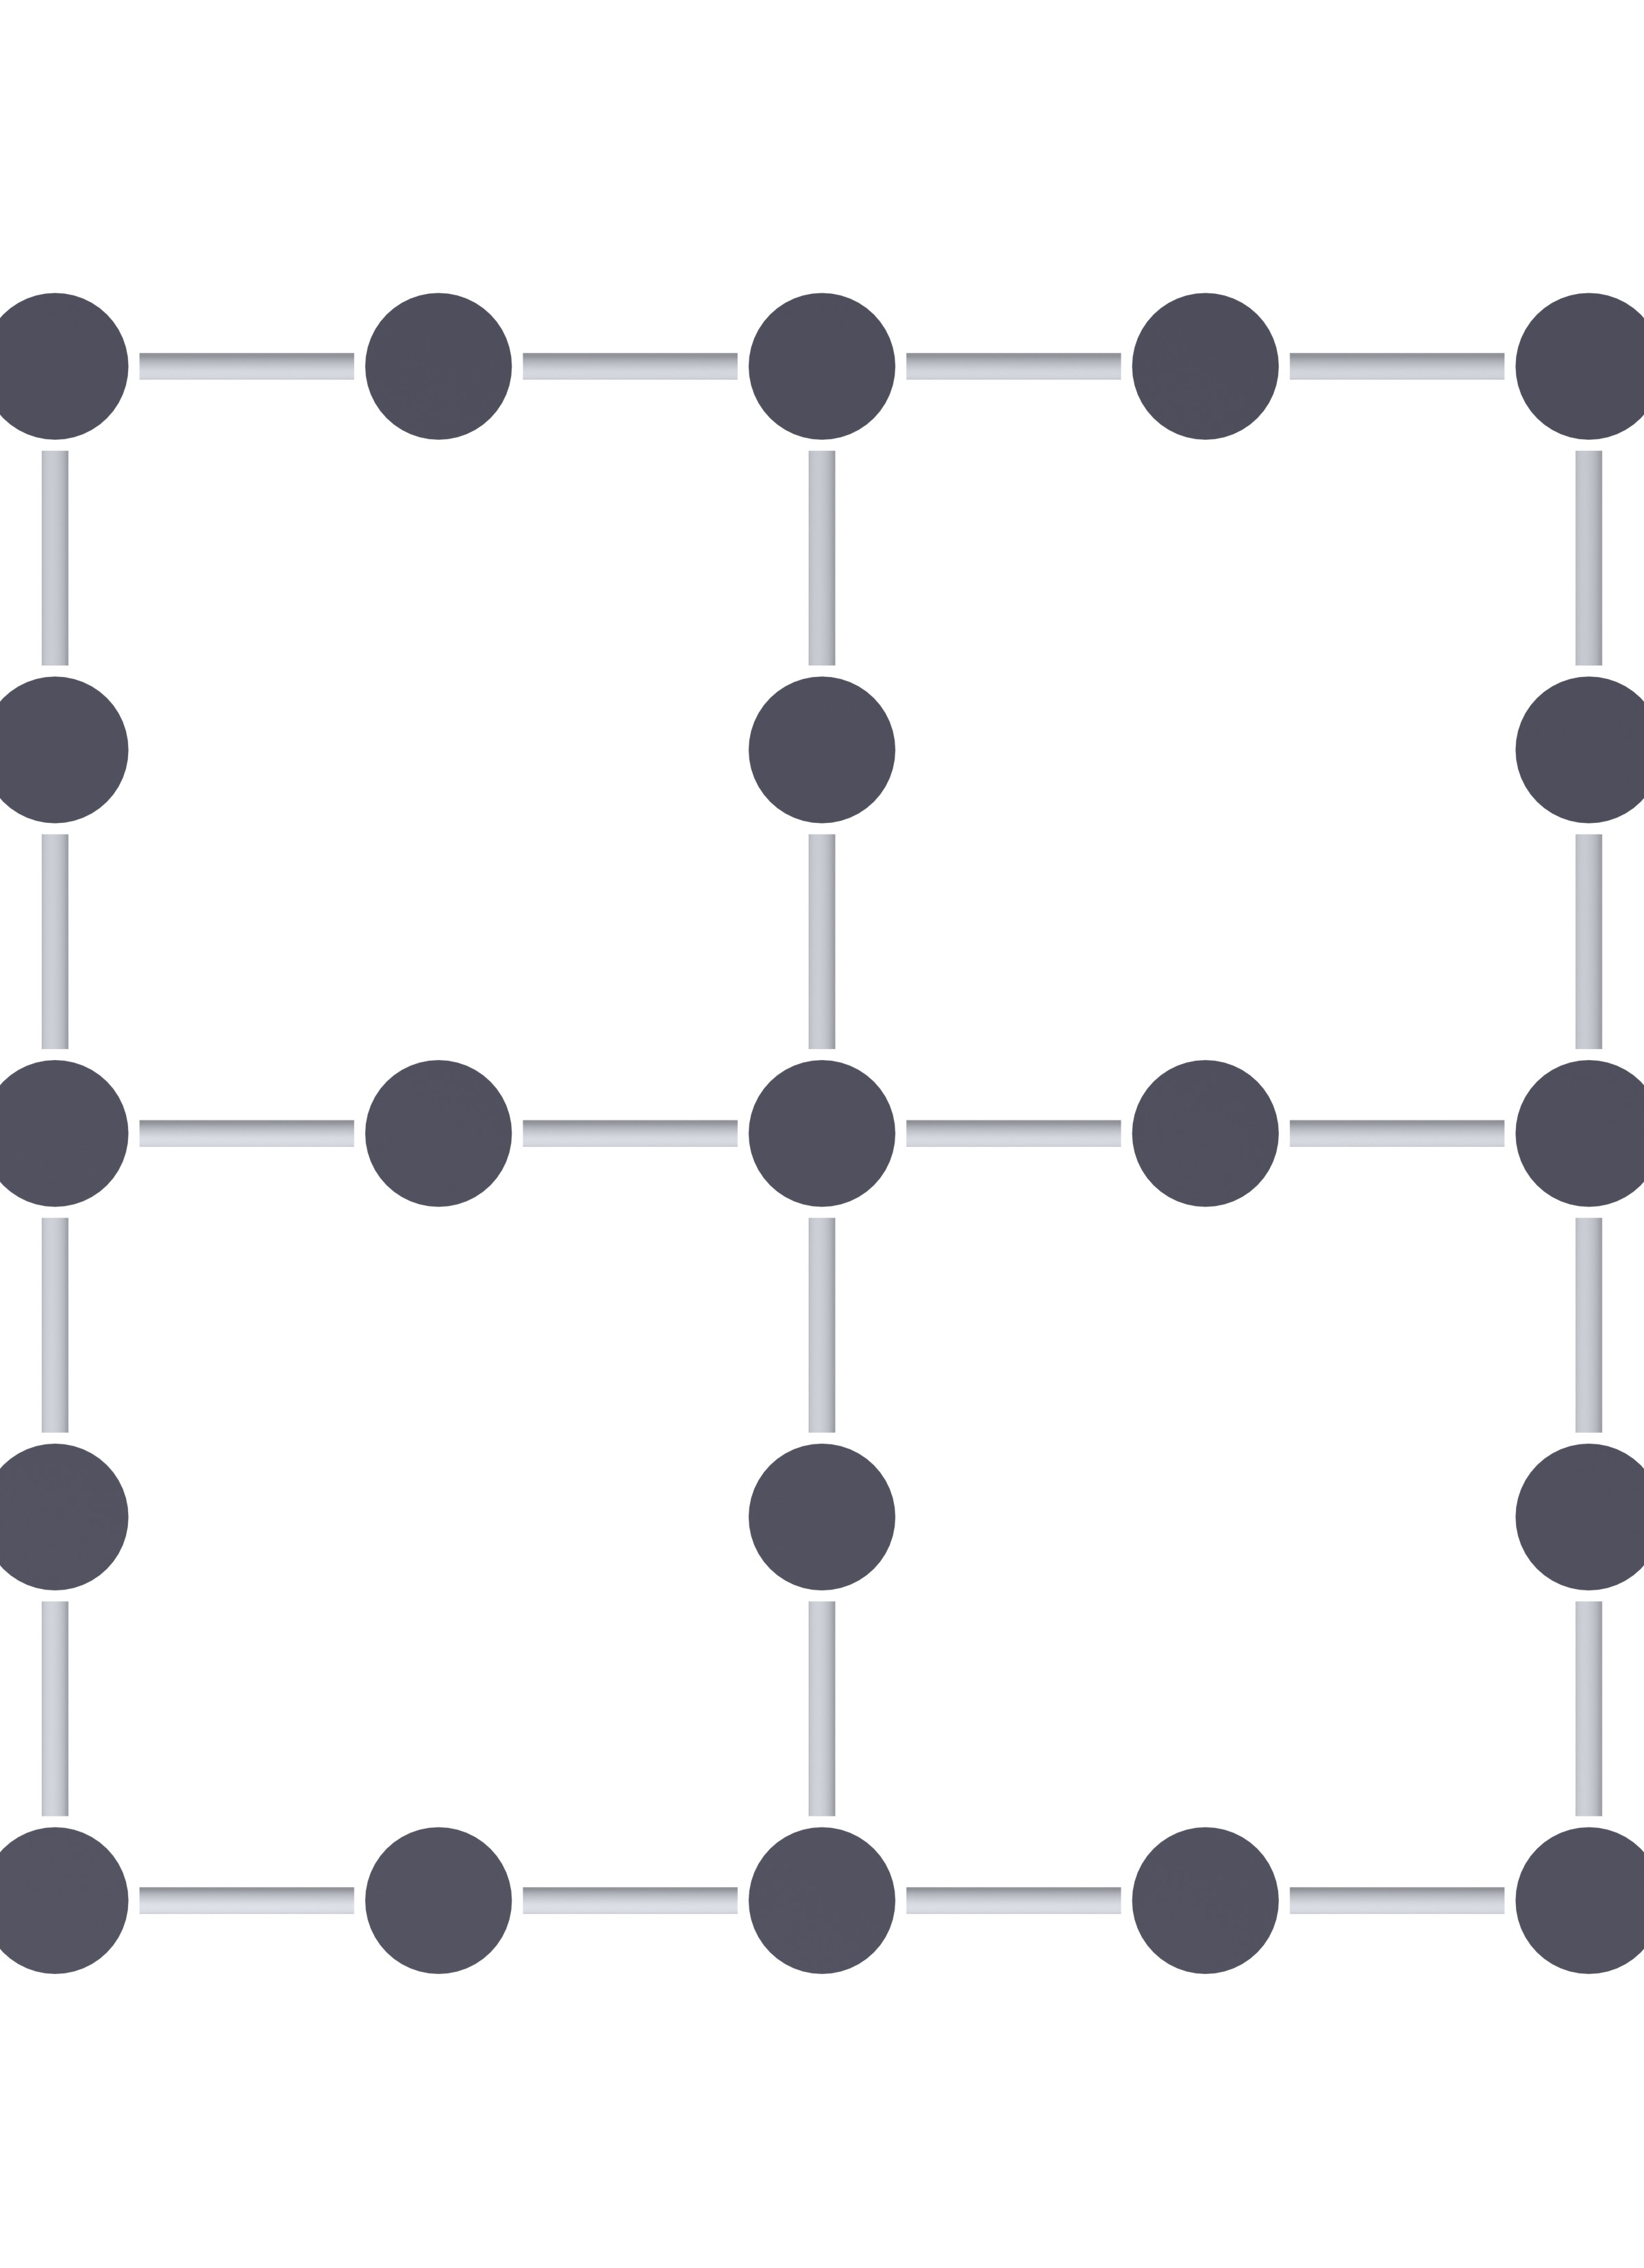
\includegraphics[width=\figw]{../blender/out/s02f05_flatbands_a.jpg}};
    % written by build_figure.sh; the painted part of the image
\path (0.0013\figw,0.1783\figw) rectangle (0.9988\figw,1.2012\figw);

    %% written by figlib.py; x and y in units of the image width
\coordinate (apanel) at (0.0335\figw,1.5214\figw);

    \node[pnl, anchor=west] at (apanel) {(a)};
  \end{scope}
  \begin{scope}[shift={(3.00cm,0)}]
    \setlength{\figw}{3.3cm}
    \node[overlay, anchor=south west, inner sep=0pt] at (0,0)
      {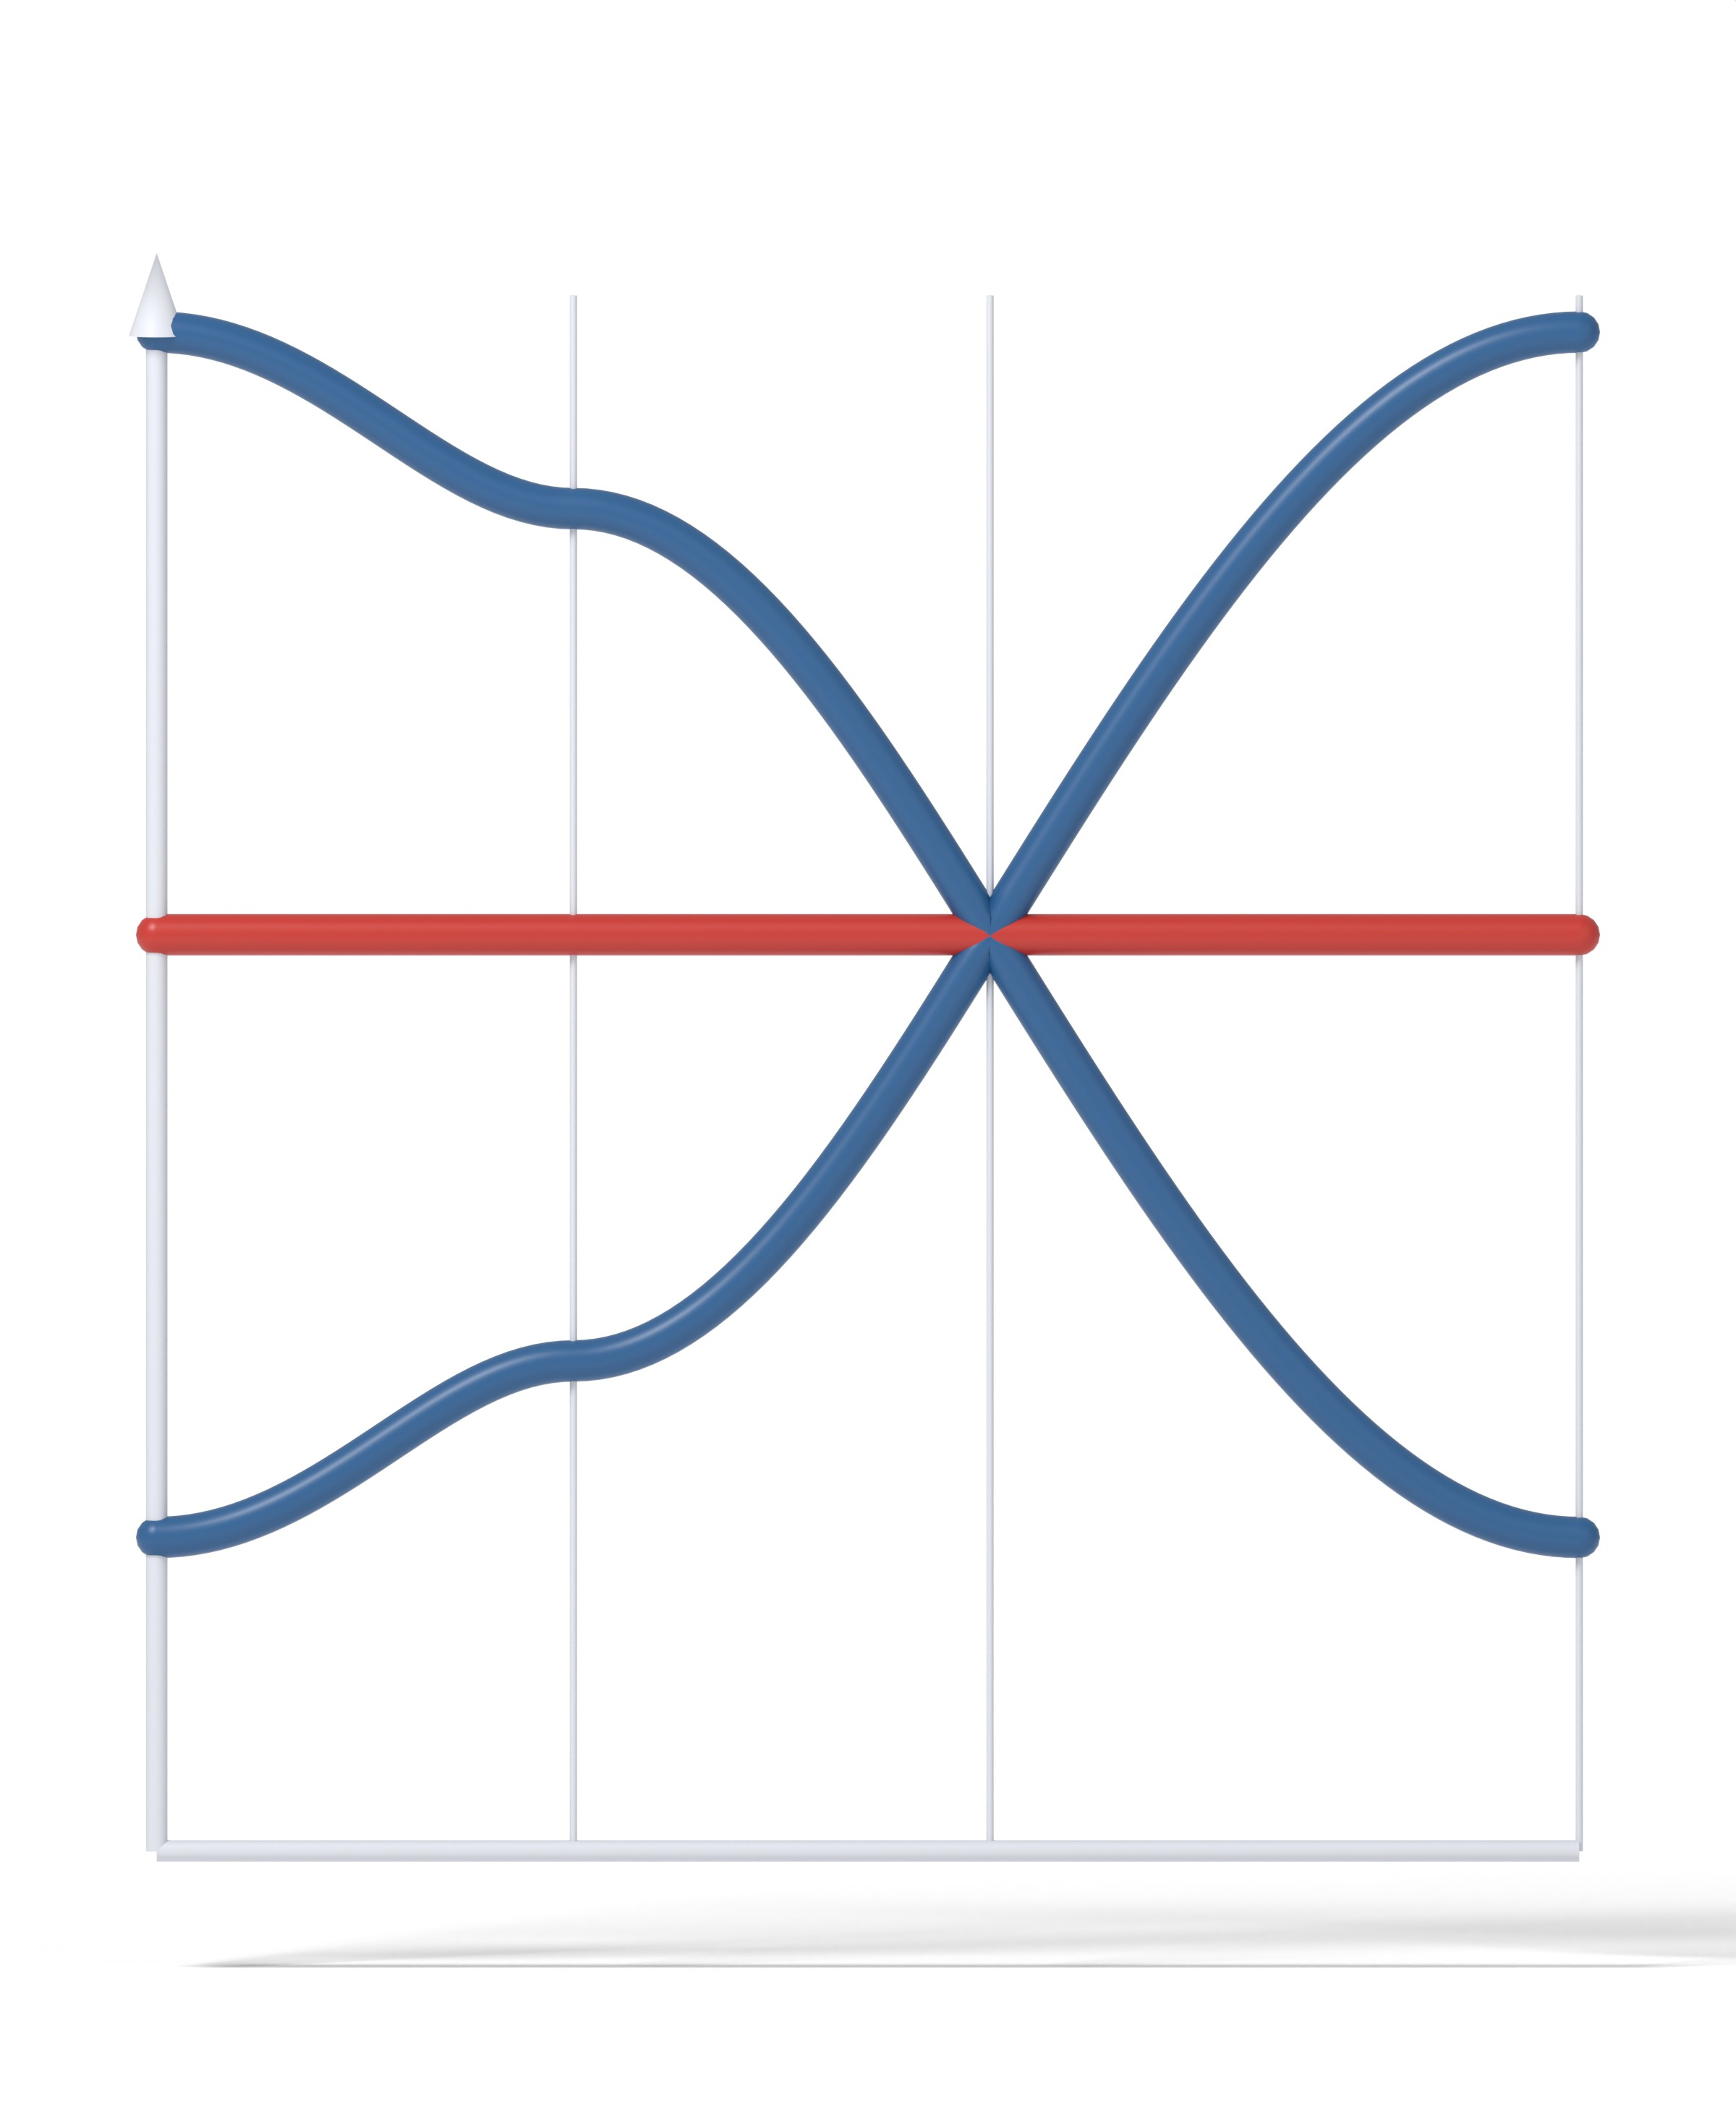
\includegraphics[width=\figw]{../blender/out/s02f05_flatbands_b.jpg}};
    % written by build_figure.sh; the painted part of the image
\path (0.0742\figw,0.0783\figw) rectangle (0.9988\figw,1.0662\figw);

    %% written by figlib.py; x and y in units of the image width
\coordinate (bG1) at (0.0903\figw,0.1396\figw);
\coordinate (bX) at (0.3303\figw,0.1396\figw);
\coordinate (bM) at (0.5703\figw,0.1396\figw);
\coordinate (bG2) at (0.9097\figw,0.1396\figw);
\coordinate (bE) at (0.0903\figw,1.0663\figw);
\coordinate (bflat) at (0.9268\figw,0.6736\figw);
\coordinate (bpanel) at (-0.0463\figw,1.1768\figw);

    \node[pnl, anchor=west, xshift=4pt] at (bpanel) {(b)};
    \node[lbl, anchor=north] at (bG1) {$\Gamma$};
    \node[lbl, anchor=north] at (bM) {$M$};
    \node[lbl, anchor=north] at (bG2) {$\Gamma$};
    \node[lbl, anchor=west] at (bE) {$\epsilon$};
    \node[lbl, anchor=north] at (bX) {$X$};
    \node[lbl, anchor=south east, yshift=1pt, text=aqmbroken] at (bflat) {$0$};
  \end{scope}
  \begin{scope}[shift={(6.40cm,0)}]
    \setlength{\figw}{2.9cm}
    \node[overlay, anchor=south west, inner sep=0pt] at (0,0)
      {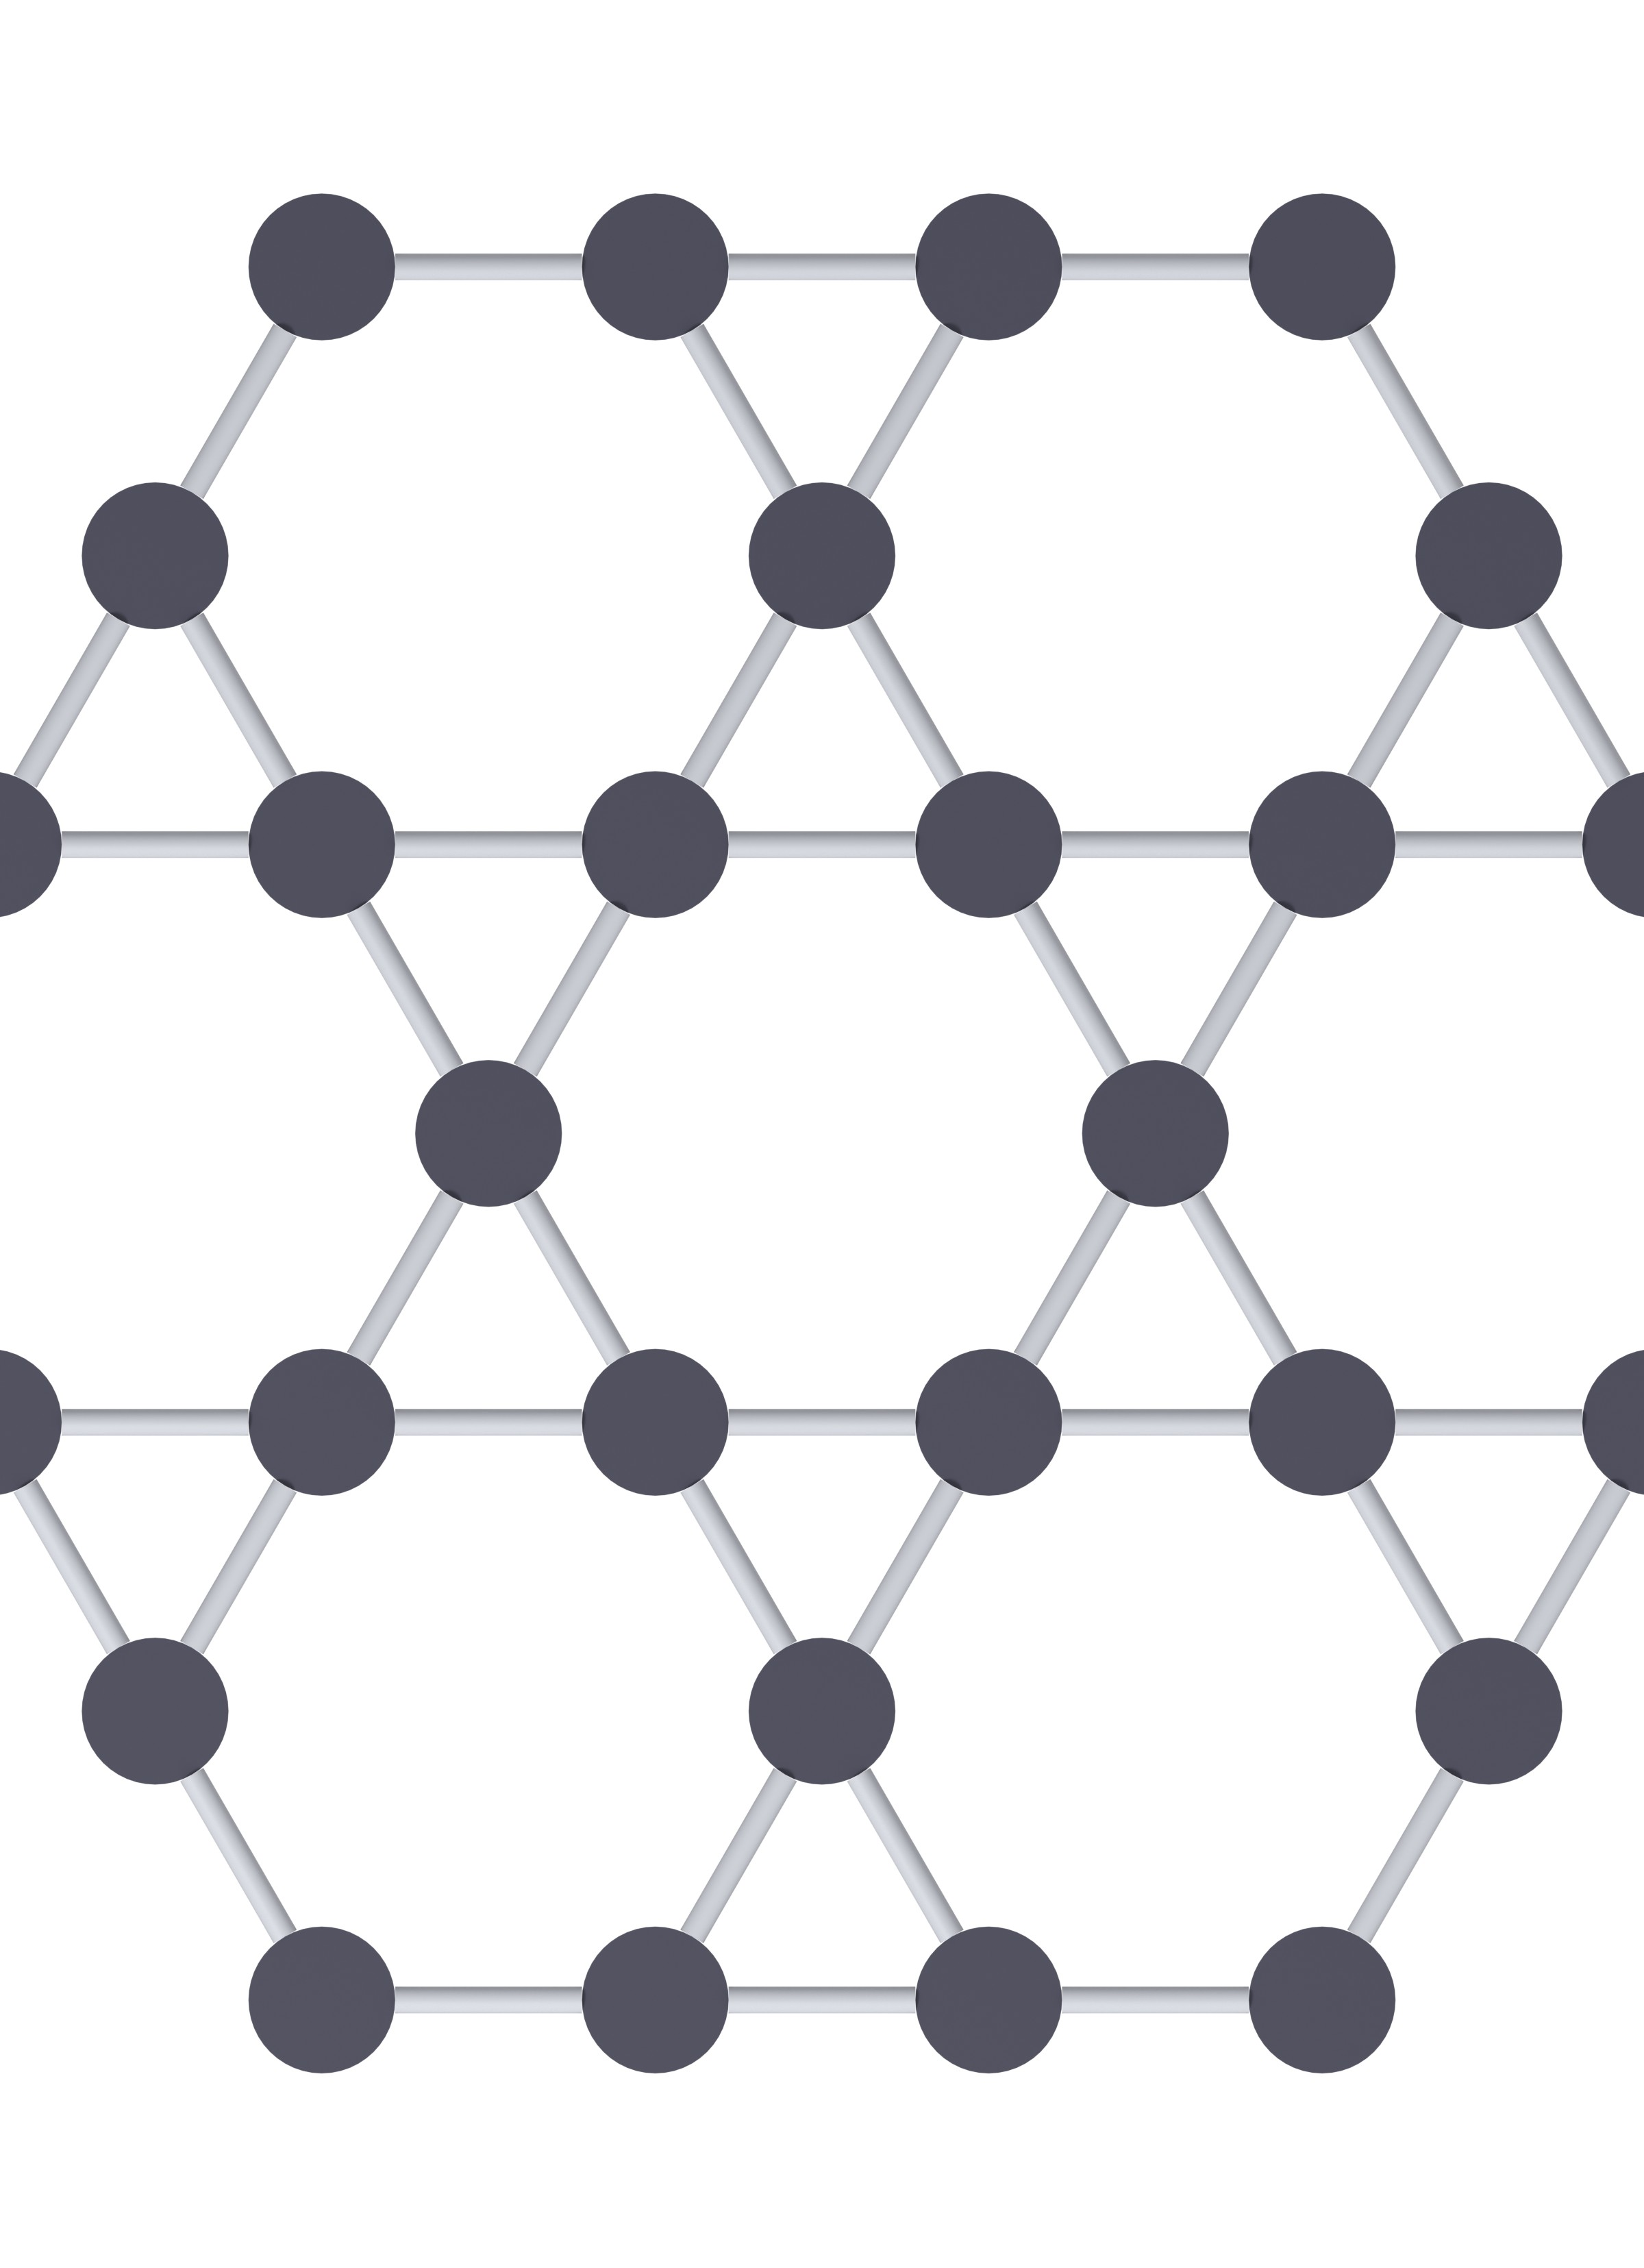
\includegraphics[width=\figw]{../blender/out/s02f05_flatbands_c.jpg}};
    % written by build_figure.sh; the painted part of the image
\path (0.0013\figw,0.1179\figw) rectangle (0.9988\figw,1.2617\figw);

    %% written by figlib.py; x and y in units of the image width
\coordinate (cpanel) at (0.0335\figw,1.5214\figw);

    \node[pnl, anchor=west] at (cpanel) {(c)};
  \end{scope}
  \begin{scope}[shift={(9.40cm,0)}]
    \setlength{\figw}{3.3cm}
    \node[overlay, anchor=south west, inner sep=0pt] at (0,0)
      {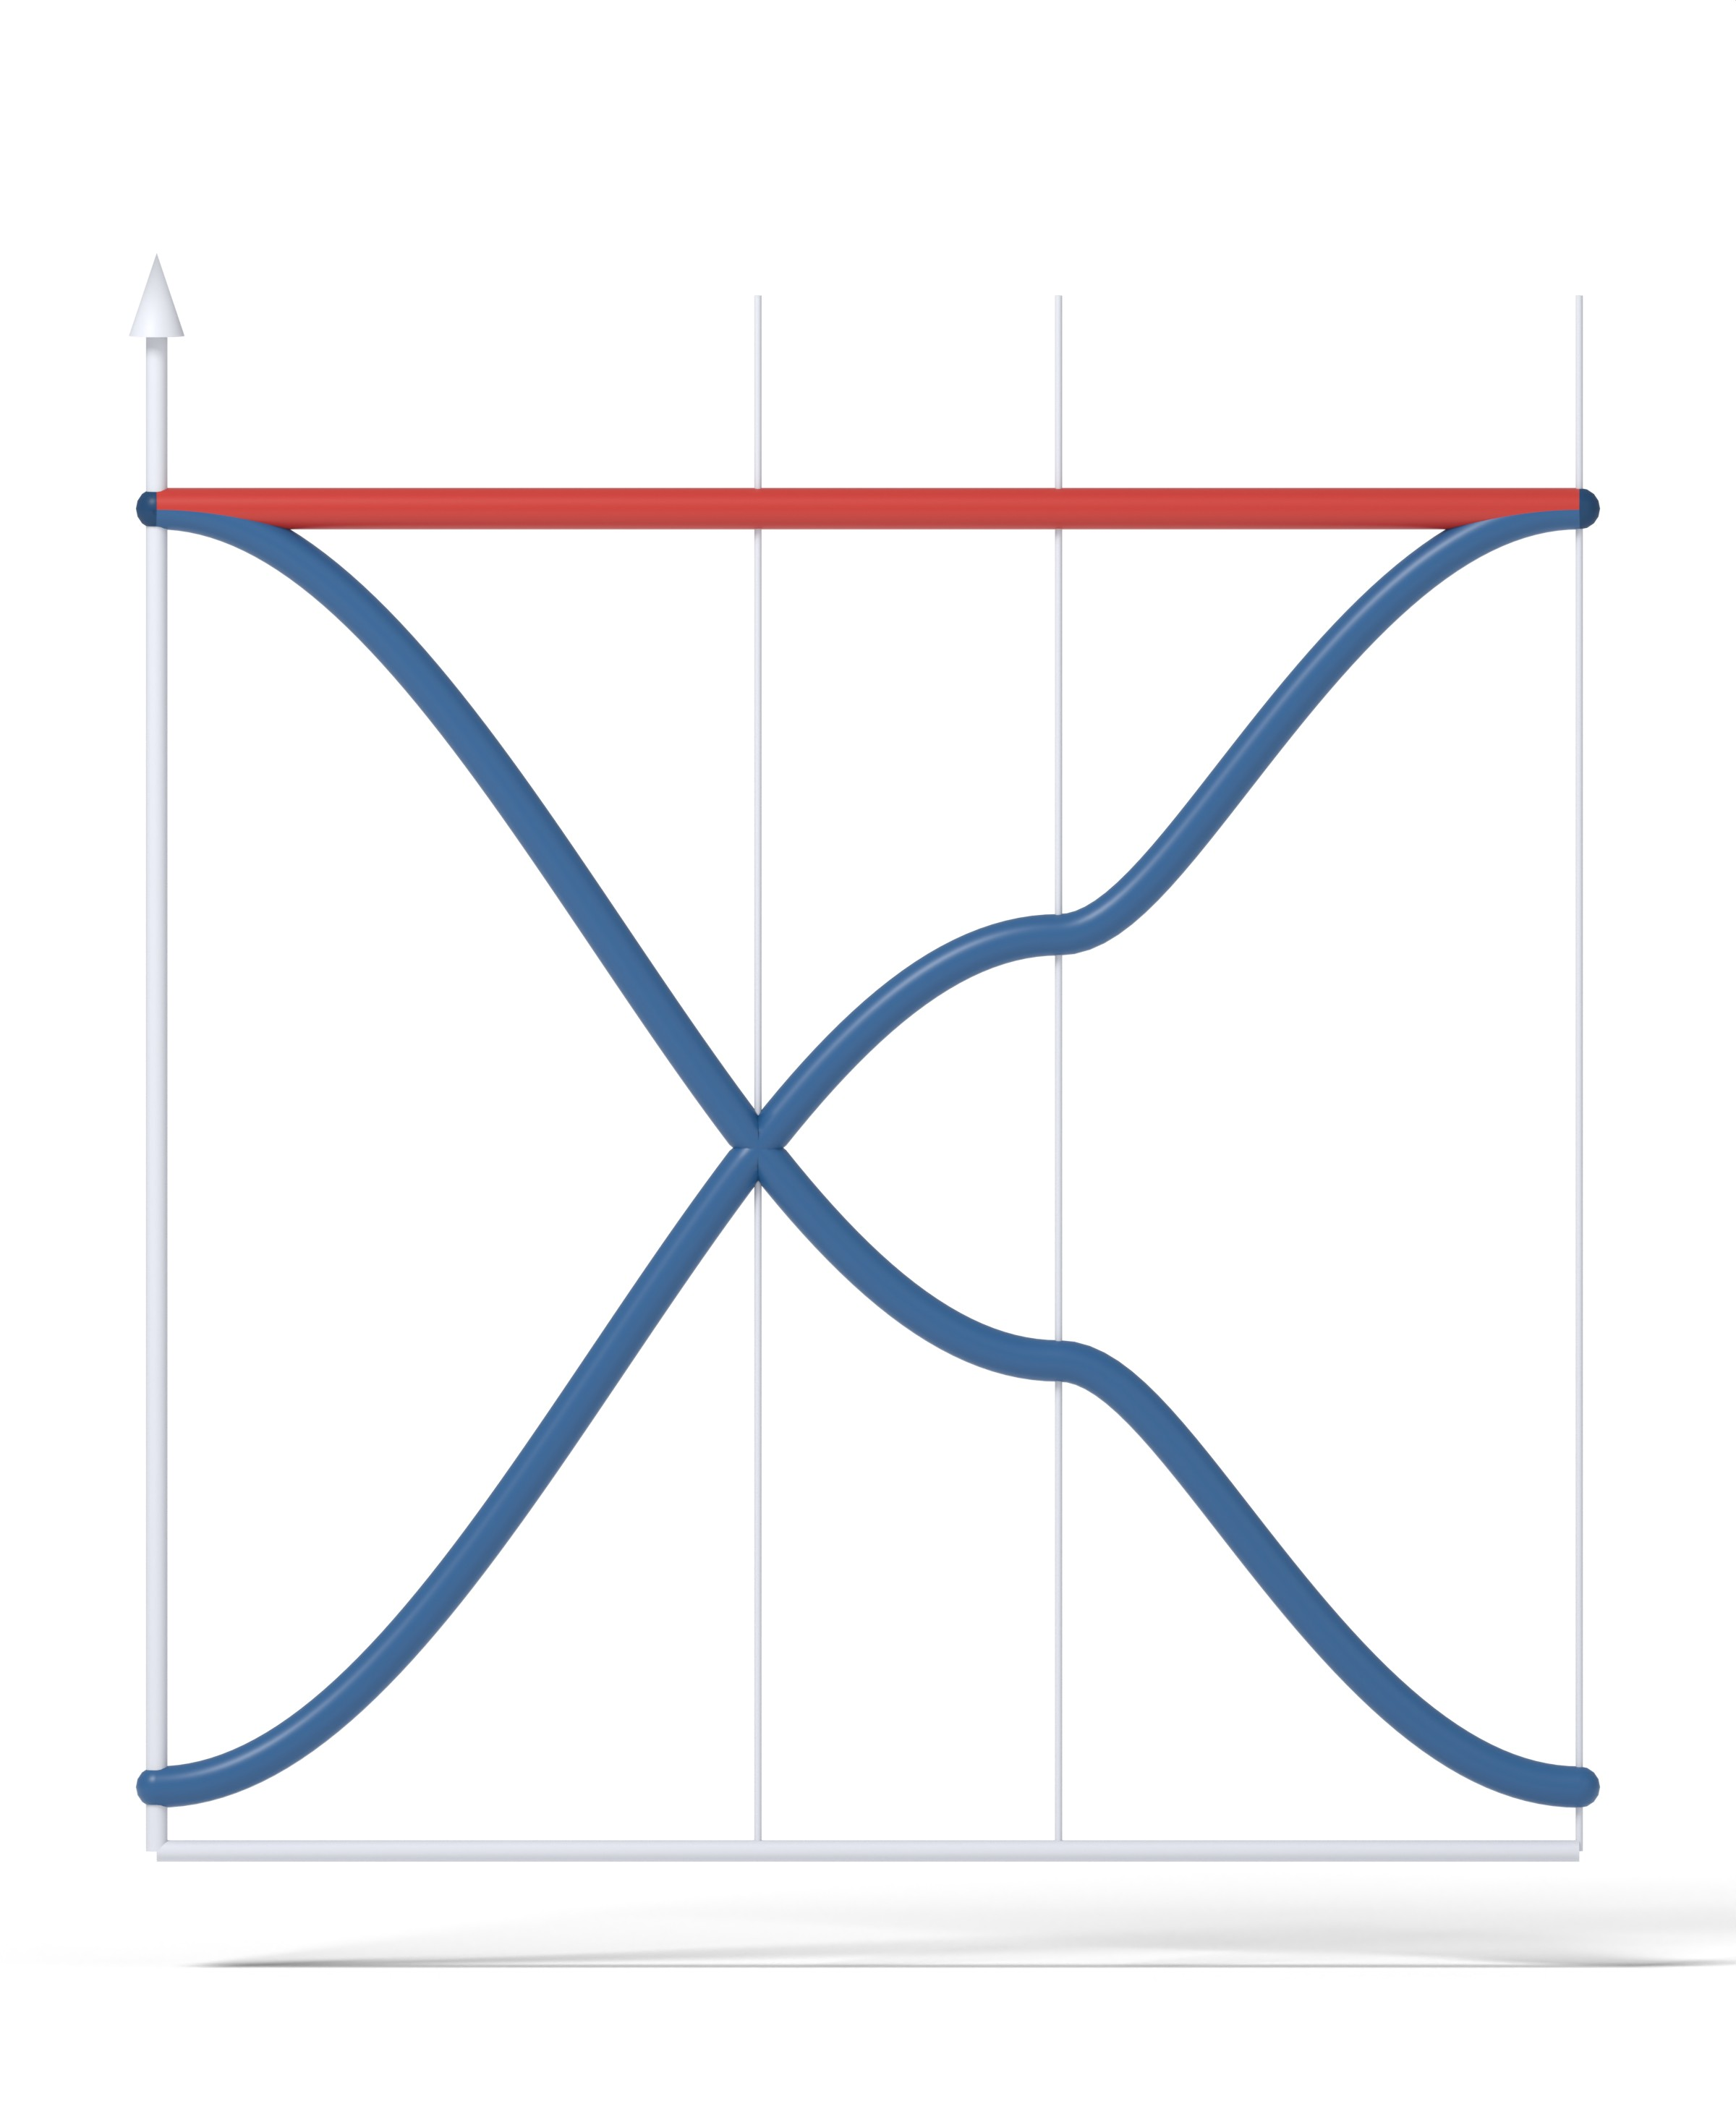
\includegraphics[width=\figw]{../blender/out/s02f05_flatbands_d.jpg}};
    % written by build_figure.sh; the painted part of the image
\path (0.0742\figw,0.0783\figw) rectangle (0.9988\figw,1.0662\figw);

    %% written by figlib.py; x and y in units of the image width
\coordinate (dG1) at (0.0903\figw,0.1396\figw);
\coordinate (dK) at (0.4366\figw,0.1396\figw);
\coordinate (dM) at (0.6098\figw,0.1396\figw);
\coordinate (dG2) at (0.9097\figw,0.1396\figw);
\coordinate (dE) at (0.0903\figw,1.0663\figw);
\coordinate (dflat) at (0.9268\figw,0.9190\figw);
\coordinate (dpanel) at (-0.0463\figw,1.1768\figw);

    \node[pnl, anchor=west, xshift=4pt] at (dpanel) {(d)};
    \node[lbl, anchor=north] at (dG1) {$\Gamma$};
    \node[lbl, anchor=north] at (dM) {$M$};
    \node[lbl, anchor=north] at (dG2) {$\Gamma$};
    \node[lbl, anchor=west] at (dE) {$\epsilon$};
    \node[lbl, anchor=north] at (dK) {$K$};
    \node[lbl, anchor=south east, yshift=1pt, text=aqmbroken] at (dflat) {$2t$};
  \end{scope}
  \begin{scope}[shift={(12.80cm,0)}]
    \setlength{\figw}{2.8cm}
    \node[overlay, anchor=south west, inner sep=0pt] at (0,0)
      {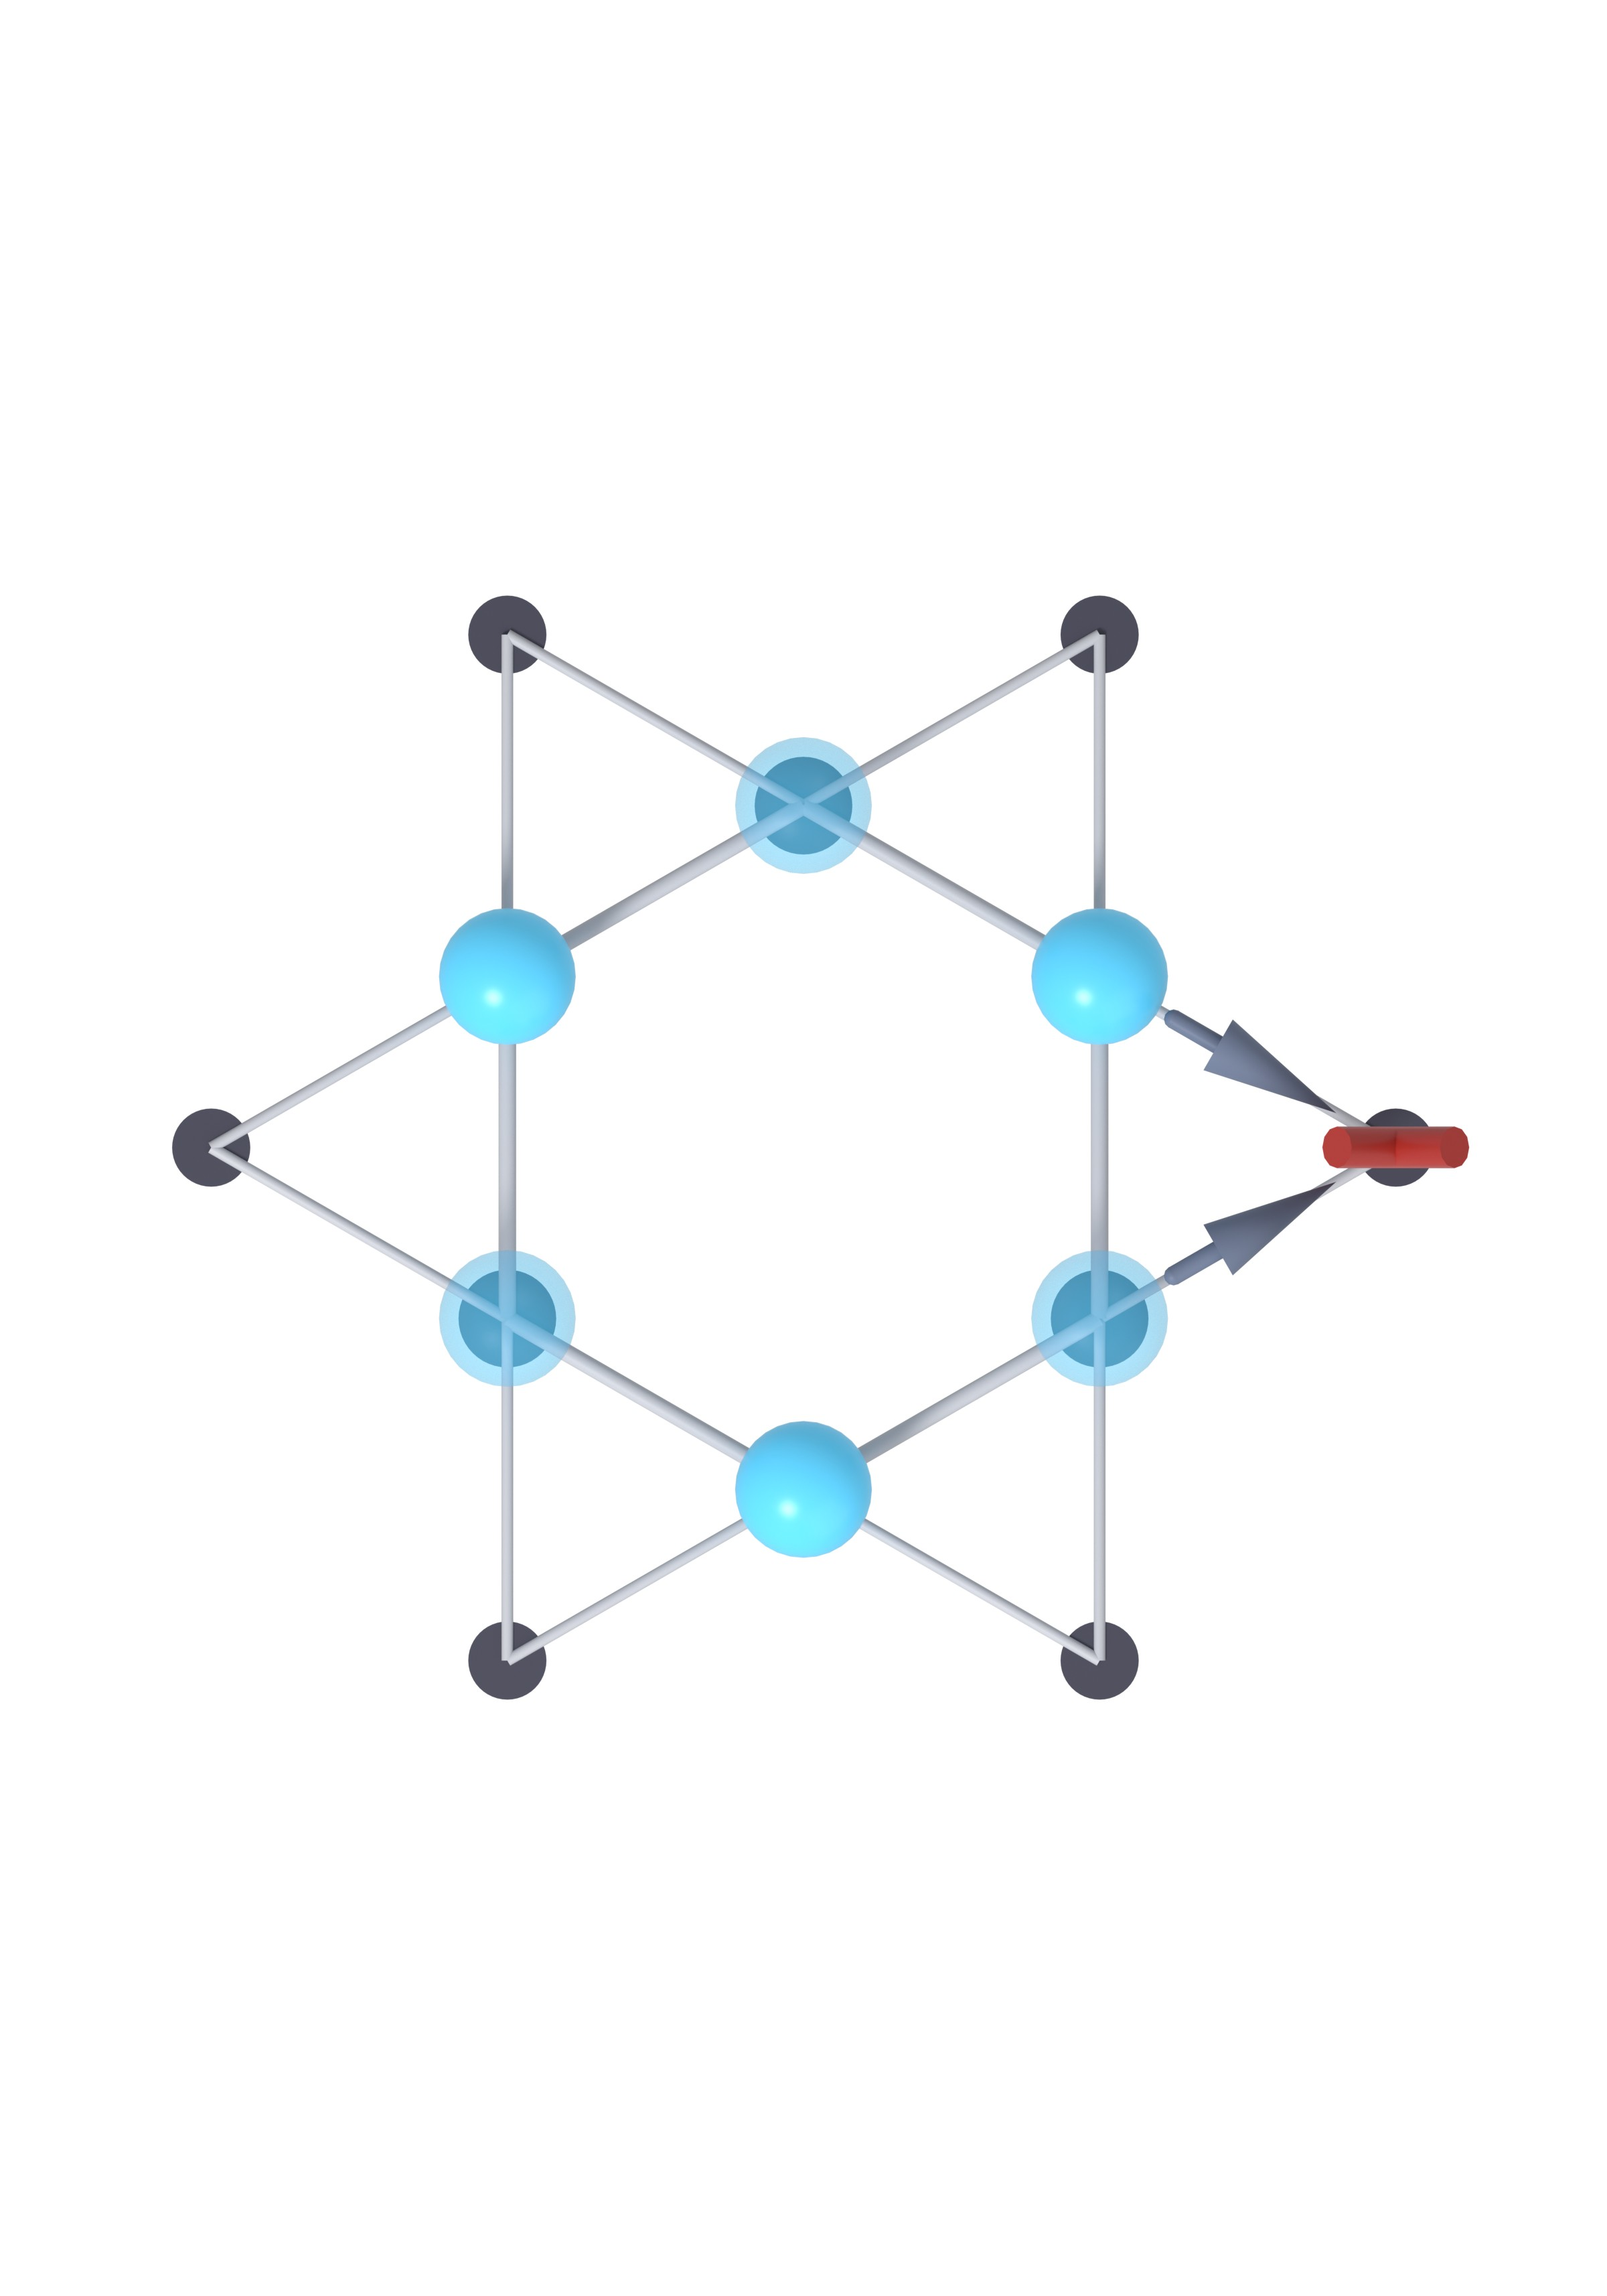
\includegraphics[width=\figw]{../blender/out/s02f05_flatbands_e.jpg}};
    % written by build_figure.sh; the painted part of the image
\path (0.1067\figw,0.3708\figw) rectangle (0.9146\figw,1.0583\figw);

    %% written by figlib.py; x and y in units of the image width
\coordinate (eamp0) at (0.7475\figw,0.8576\figw);
\coordinate (eamp1) at (0.5000\figw,1.0005\figw);
\coordinate (eamp2) at (0.2525\figw,0.8576\figw);
\coordinate (eamp3) at (0.2525\figw,0.5718\figw);
\coordinate (eamp4) at (0.5000\figw,0.4290\figw);
\coordinate (eamp5) at (0.7475\figw,0.5718\figw);
\coordinate (ezero) at (0.9294\figw,0.7148\figw);
\coordinate (epanel) at (0.0288\figw,1.3687\figw);

    \node[pnl, anchor=west] at (epanel) {(e)};
    \node[lbl, anchor=south west, xshift=-3pt, yshift=1pt] at (eamp0) {$+$};
    \node[lbl, anchor=north west, xshift=-3pt, yshift=-1pt] at (eamp5) {$-$};
  \end{scope}
\end{tikzpicture}
\end{document}
